
\documentclass[letterpaper, 10 pt, conference]{ieeeconf}  % Comment this line out if you need a paper

%\documentclass[a4paper, 10pt, conference]{ieeeconf}      % Use this line for a4 paper

\IEEEoverridecommandlockouts

\overrideIEEEmargins                                      % Needed to meet printer requirements.

% See the \addtolength command later in the file to balance the column lengths
% on the last page of the document
\usepackage{cite}
% The following packages can be found on http:\\www.ctan.org
\usepackage{graphicx} % for pdf, bitmapped graphics files
%\usepackage{epsfig} % for postscript graphics files
%\usepackage{mathptmx} % assumes new font selection scheme installed
%\usepackage{times} % assumes new font selection scheme installed
\usepackage{amsmath} % assumes amsmath package installed
\usepackage{amssymb}  % assumes amsmath package installed
\usepackage{math}
\usepackage{aircraftshapes}
\usepackage[caption=false]{subfig} % subfigures.  false option prevents conflicts in caption styling with other packages
%\usepackage{natbib}
%\usepackage{standalone}
\usepackage{tikz}
\usetikzlibrary{positioning}
\usetikzlibrary{shapes,arrows}
\tikzstyle{pre}=[<-,>=stealth,thick]
\tikzstyle{post}=[->,>=stealth,thick]
\tikzstyle{prepost}=[<->,>=stealth,thick]
\usetikzlibrary{automata,positioning,graphs,calc}

\usepackage{graphicx}
\usepackage{color}
\usepackage{pgfplots}
\pgfplotsset{compat=1.15}
\usepackage{pgf-umlsd}
\usepackage{ifthen}
\usepackage{graphicx}
\usepackage{hyperref}
\usepackage{cleveref}


\usepackage[ruled,longend,linesnumbered]{algorithm2e}
%
%\RequirePackage{fix-cm}

\usepackage{pgfplots}
% \usepackage{fancyhdr}
% \pagesty

\usepackage{xcolor}
\newcommand{\todo}[1]{{\color{blue}[TODO: #1]}}
\newcommand{\response}[1]{{\color{green}[RESPONSE: #1]}}

\title{\LARGE \bf
	Evolutionary Nonlinear Model Predictive Control \\ on a Fixed-Wing and Multirotor
}

%\titlerunning{Short form of title}        % if too long for running head

\author{Jaron Ellingson$^{1}$, Mat Haskell$^{2}$%
%	\thanks{*This material is based upon work supported by the National Science Foundation under Grant No. 1727010. This work is also supported by the Center for Unmanned Aircraft Systems (C-UAS), a National Science Foundation Industry/University Cooperative Research Center (I/UCRC) under NSF award No. IIP-1161036 along with significant contributions from C-UAS industry members.}% <-this % stops a space
	\thanks{$^{1}$ Jaron Ellingson is an MS candidate in the Department of Mechanical Engineering, Brigham Young University
		{\tt\small jaronce@byu.eduu}}%
	\thanks{$^{2}$ Mat Haskell is a PhD candidate in the Department of Mechanical Engineering, Brigham Young University
		{\tt\small mathew.haskell@byu.edu}}%
}

\begin{document}
\maketitle
\thispagestyle{empty}
\pagestyle{empty}

\date{Received: date / Accepted: date}
% The correct dates will be entered by the editor


\maketitle

\begin{abstract}
Real-time model predictive control (MPC) is limited to short time horizons and linear systems because the optimization complexity is too large with long time horizons and nonlinear systems. For this reason, MPC is typically accomplished using linearized models and convex optimization solvers. We seek to explore evolutionary algorithms allowing for nonlinear models and constraints, non-convex costs, and extended time horizons.

Our contributions include extending nonlinear evolutionary MPC to flight vehicles, fixed-wing and multirotor UAVs, as well as enhancing the evolutionary algorithm. We also intend to parameterize the design space of the optimization to reduce solve times. These contributions will validate the robust and effective nature of the algorithm.

% \PACS{PACS code1 \and PACS code2 \and more}
% \subclass{MSC code1 \and MSC code2 \and more}
\end{abstract}

%\section{Project Direction}


%Real-time model predictive control (MPC) is limited to short time horizons and linear systems because the optimization complexity is too large with long time horizons and nonlinear systems. For this reason, MPC is typically accomplished using linearized models and convex optimization solvers. We seek to explore evolutionary algorithms allowing for nonlinear models and constraints, non-convex costs, and extended time horizons. 

%This work is a continuation of the work accomplished in \cite{hyatt2020parameterized} which is developed to parameterize long time horizons. Our contributions include extending nonlinear evolutionary MPC to flight vehicles, fixed-wing and multirotor UAVs, as well as enhancing the evolutionary algorithm. We also intend to parameterize the design space of the optimization to reduce solve times. These contributions will validate the robust and effective nature of the algorithm.

%While parallelization of the evolutionary algorithm allows for real-time control, writing the code to parallelize the algorithm might be out of the scope for this project. A neural network is used in the NEMPC algorithm in \cite{hyatt2019real}, which interfaced with the GPU under the hood. This work seeks to implement NEMPC without using a neural network, making parallelization more difficult.


\section{Introduction}

In \cite{hyatt2017real}, linear MPC was performed in real-time on a robotic arm using an evolutionary optimization algorithm rather than a typical convex solver. To make the algorithm real-time, each state propagation in the evolutionary algorithm during a single generation occurred in parallel on a graphics processing unit (GPU). GPU's are known to be fast at matrix multiplications, which the linearized model provided.

The previous work using an evolutionary algorithm was continued in \cite{hyatt2019real} where nonlinear dynamics were used as the model for real-time MPC. The key change in this work from \cite{hyatt2017real} is that the nonlinear dynamics were approximated using a neural network. The neural network was able to learn the nonlinear dynamics in a way that still utilized matrix multiplications, allowing for parallelization of the genetic algorithm on a GPU.

In \cite{hyatt2020parameterized}, the evolutionary MPC algorithm is compared to a MPC using a QP solver both with a parameterized optimization design space to reduce the number of design variables. Both algorithms are capable of real-time control of nonlinear robotic arms. With MPC, the optimization design variable is the future trajectory of control inputs that should be applied to the system over a finite time horizon. This work used a piece-wise linear function to parameterize the trajectory of future inputs, usually with only 2 lines (3 points). This allowed for a significant reduction in the search space of the optimization and thus, faster solve times. With the parameterization, the solve times of both algorithms are capable of running control at over 100 Hz. MPC using the QP solver was still faster than the parallelized NEMPC, but the evolutionary algorithm allows for a nonlinear model.

\section{Model Predictive Control}


The MPC problem is formulated by

\begin{equation}
\label{eq:objective}
\begin{aligned}
\text{minimizing} & \quad J= \sum_{k=0}^{T-1} (f(\mathbf{x}_k,\mathbf{u}_k)-\mathbf{x}_{d})^{\top} Q (f(\mathbf{x}_k,\mathbf{u}_k)-\mathbf{x}_{d}) \\
\text{with respect to} & \quad \mathbf{u}_k  \\
\text{subject to} & \quad \mathbf{L}_b \le \mathbf{u}_k \le \mathbf{U}_b, \\
\end{aligned}
\end{equation}


where $f(\mathbf{x}_k,\mathbf{u}_k)$ represents the nonlinear dynamics of a wither the quadrotor or fixed-wing aircraft applied with Runge-Kutta 4th order approximation. $\mathbf{x}_k$ and $\mathbf{x}_{d}$ are our calculated state and desired state, $\mathbf{u}_k$ represents our inputs, and $\mathbf{L}_b$ and $\mathbf{U}_b$ are our lower and upper bounds on the inputs. Finally, the diagonal matrix $Q$ represents a cost weighting matrix associated with each state. In \cref{subsub:quad,subsub:fw} we will highlight the differences between the quadrotor and fixed-wing states, desired state, inputs, and cost matrix.

-Optimize time window of control inputs

-Predict future states and compute error with desired states

-Quadratic cost on error

-Apply 1st set of inputs and resolve problem at next time 
step (model isn't perfect)



\section{Evolutionary Algorithm}

Most of the work which has been accomplished on our evolutionary algorithm developement was inspired by or implemented from \cite{martins2017multidisciplinary}.

\subsection{Initialization}

I initialize our first population, we choose to implement a Latin-Hypercube sampling algorithm to optimize starting coverage of the design space. We also decided to insert 1 sample at equilibrium because we know that optimal solutions will lay near equilibrium, especially at level or minimal movement flight. 

-LHS for initial population generation

-Also add in 1 sample for equilibrium

-Lot of time can be spent at equilibrium

-Finds this solution immediately

-Can add slew rate \todo{I thought we had this but didn't really keep it.}

-Enforce saturation (bound constraints)


\subsection{Fitness}

To evaluate the fitness of each 

-RK4 integration of dynamics for f(x,u)

-Q is positive definite diagonal matrix

-Design variables are only $u_k$ vectors

-Large reduction of order

-Dim = m*N rather than (m+n)*n

-With N = 10 and m = 4 gives 40 design variables



\subsubsection{Quadrotor Fitness}
\label{subsub:quad}

\subsubsection{Fixed-Wing Fitness}
\label{subsub:fw}



where $f(\mathbf{x}_k,\mathbf{u}_k)$ represents the nonlinear dynamics of a fixed wing aircraft applied with Runge-Kutta 4th order approximation (see Appendix \ref{sec:dynamics} for more details). $\mathbf{x}_k$ and $\mathbf{x}_{d}$ are our calculated state and desired state where,

\begin{equation}
\label{eq:lqr_current_desired_states}
\mathbf{x}=\begin{bmatrix}\mathbf{p} \\ \mathbf{v} \\ \mathbf{q} \\ \boldsymbol{\omega}\end{bmatrix}.
\end{equation}

Furthermore, $Q$ is our cost matrix and initialized as,

\begin{equation}
Q = \text{diagonal}(\begin{bmatrix}
0,0,100,1,0,0,50,50,50,0,0,0
\end{bmatrix}).
\end{equation}

I choose this particular cost because I don't necessarily want the aircraft to hit a particular location but to maintain a desired altitude and heading while also maintaining a desired forward velocity. This can be seen in \Cref{fig:vet_field} where the aircraft is some distance away from the the direct path from $w_{i-1}$ to $w_i$. \Cref{fig:vet_field} also shows a vector field which slowly places the aircraft onto a course to the next waypoint. This vector field allows us to define the commanded heading of the aircraft as we are far away from the desired path. this vector field is defined as,

\begin{equation}
\check{\chi}=\chi_{l}-\chi_{\infty}\frac{2}{\pi}\tan^{-1}\left(k_{\chi}\mathbf{e}_{2}\right),
\end{equation}

where $\chi_l$ is the course angle of our line, and $\check{\chi}$ is the desired course angle. Furthermore, $k_\chi$ is a positive gain and $\chi_\infty$ is the maximum allowed difference between $\check{\chi}$ and $\chi_l$.


\begin{figure}
	\centering
	\begin{tikzpicture}
	\def\length{sqrt(1+(-pi/6*2/pi * atan(0.1*x))^2)}
	\begin{axis}[
	title={},
	domain=-2:2,
	view={0}{90},
	axis background/.style={fill=white},
	xticklabels={},
	yticklabels={},
	ticks=none,
	]
	\addplot3[black,
	quiver={
		u={-pi/6*2/pi * atan(0.1*x)/\length},
		v={1/\length},
		scale arrows=0.3,
	},
	-stealth,samples=15]
	{x};
	\end{axis}
	%\draw [very thick][-latex](160pt,20pt)..controls(100pt,25pt) and (60pt,45pt)..(42pt,58pt);
	%\filldraw(160pt,20pt)circle(2pt) (100pt,25pt)circle (2pt) (60pt,45pt)circle (2pt) (42pt,58pt)circle (2pt);
	\coordinate[label = above:$w_{i}$] (wi) at (97.5pt,161pt);
	\node at (wi)[circle,fill,inner sep=2.5pt]{};
	\coordinate[label = below:$w_{i-1}$] (wi1) at (97.5pt,0pt);
	\node at (wi1)[circle,fill,inner sep=2.5pt]{};
	\draw[very thick] (wi1) -- (wi);
	
	\draw [line width=2pt, dash pattern=on \pgflinewidth off 2pt] plot [smooth, tension=0.75] coordinates {(140pt,37pt) (105pt,60pt) (97.5pt,100pt)};
	\node [aircraft top,fill=black,minimum width=0.75cm,rotate=160] at (150pt,33.5pt) {};
	
	%\filldraw(97.5pt,161pt)circle(2pt) (97.5pt,0pt)circle(2pt);
	%\draw[very thick] (97.5pt,161pt) -- (97.5pt,0pt);
	\end{tikzpicture}
	\caption{A vector field which converges onto a path from one waypoint to another.}
	\label{fig:vet_field}
	
\end{figure}




My design variables $\mathbf{u}_k =\begin{bmatrix}s_{a} & s_{e} & s_{t} & s_{r}\end{bmatrix}^{\top}$ represent the control inputs to the system and are constrained to be within certain bounds. The aileron, elevator, and rudder are all constrained to be within $-\pi/2$ to $\pi/2$ radians and the throttle is constrained from 0 to 1. To reduce the number of design variables, I choose to have the inputs applied along a segment of the trajectory and do not choose a new input at every time step. 

%I choose to have 10 control inputs for a time horizon of 1 second with time steps of 0.01 seconds. This means every 0.1 seconds I apply a new control input. \Cref{fig:sub2,fig:cd2} shows only 10 inputs applies over the trajectory of 1 second for two separate test cases.

\begin{figure*}[htbp]
	\centering
	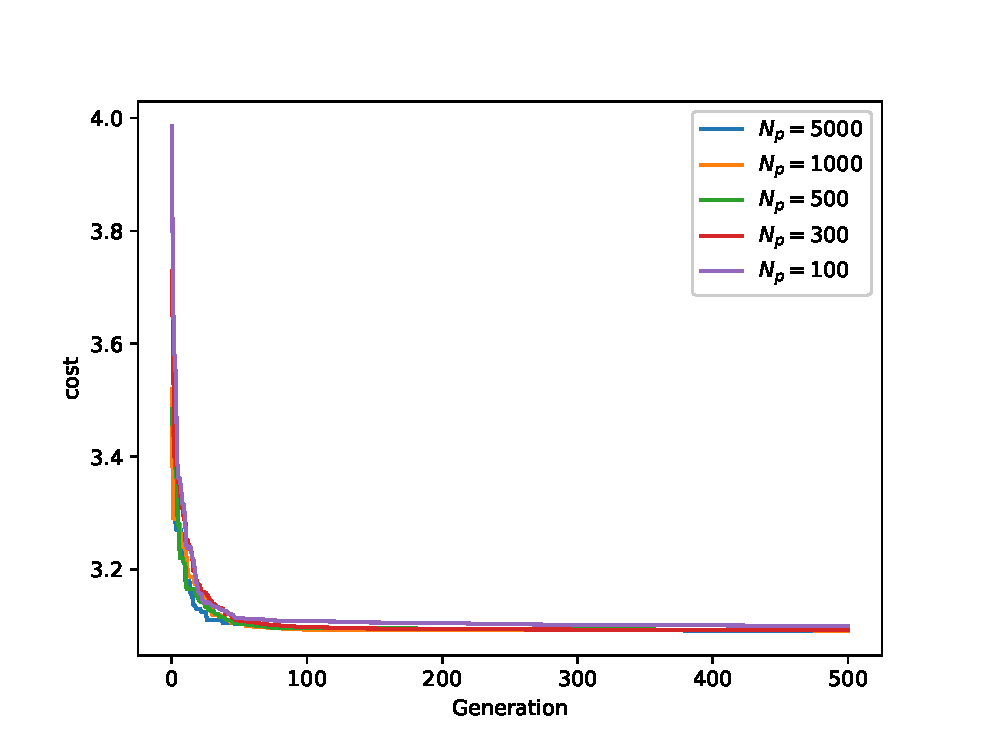
\includegraphics[width=0.45\textwidth]{figures/fixedwing_convergence.eps}
	\caption{Fixed-wing convergence.}
	\label{fig:fw_convergence}
\end{figure*}


\subsection{Selection}

-Tried keeping top percentage

--Match with equal amount of strangers to prevent stagnation

--Yields small mating pool

-Tried tournament from textbook

--Randomly pair off all members of population twice, keeping winners

--Mating pool is same size as population


\subsection{Crossover}

-Tried randomly picking genes from parents one by one

-Randomly flip a coin for each design variable

-Tried linear crossover

-xc1 = 0.5xp1 + 0.5xp2

-xc2 = 2xp1 - xp2


\subsection{Mutation}

-Tried mutating entire members of the population with low probability

-Tried mutating each individual gene of each member of the population individually with low probability

-Mutations were adding a small amount of gaussian noise


\subsection{Warmstart}

-Assume that optimal input won’t vary much from time step to time step

-Run 200 (or any number) of generations the first time solving

-After the first time, use the population from the previous time step as the starting point and only run again for 1 generation

-Don’t randomly initialize the population every time
First solve takes longer, but can be real-time afterwards


\section{Results}


\begin{figure*}[htbp]
	\centering
	\subfloat[]{
		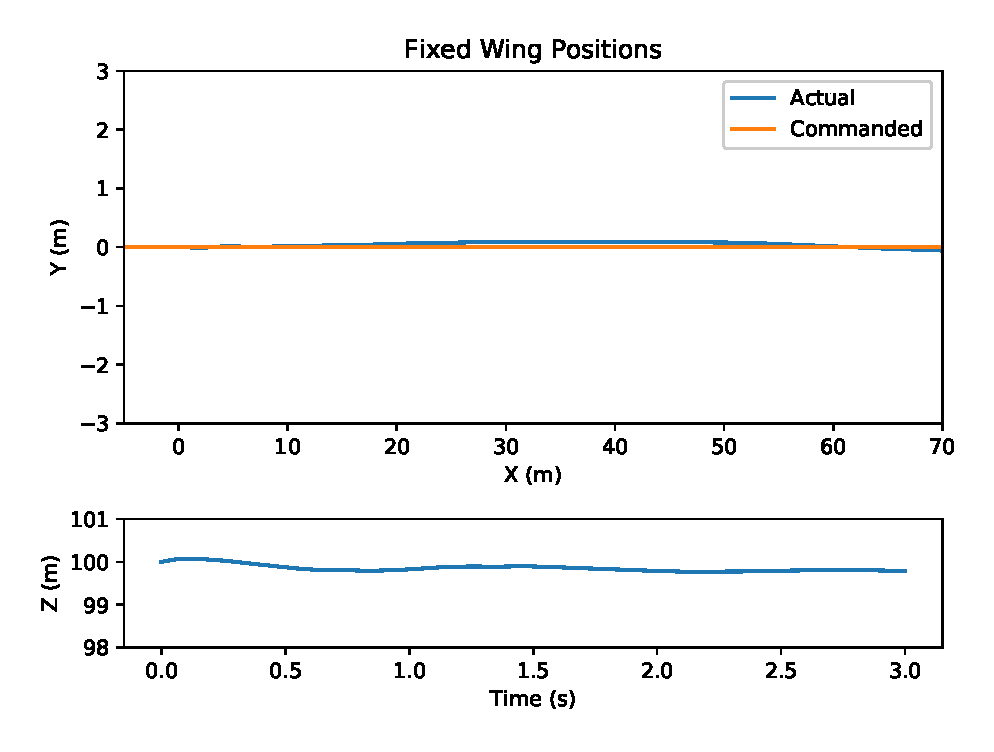
\includegraphics[width=0.45\textwidth]{figures/fixedwing_positions.eps}
		\label{fig:fw_positions_level}
	}
	\qquad
	\subfloat[]{
		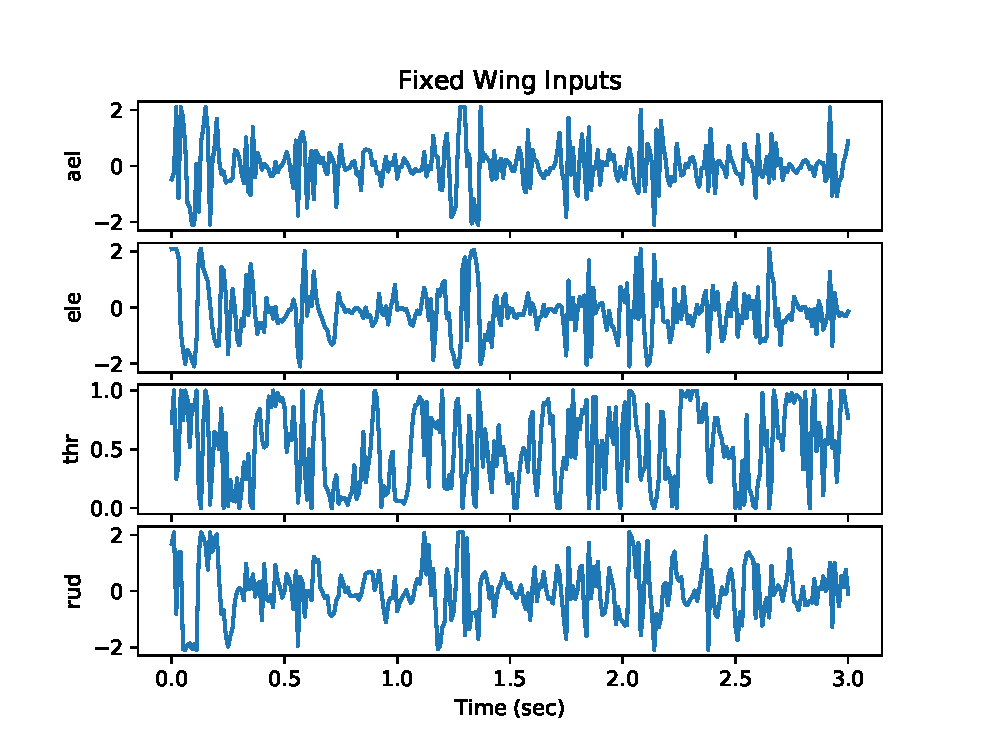
\includegraphics[width=0.45\textwidth]{figures/fixedwing_inputs.eps}
		\label{fig:fw_input_level}
	}
	\caption{Case 1 is the optimization of the aircraft in level flight. The aircraft started at the point (0,0,100) and was commanded to maintain the course on the commanded straight line. It took 37.45 seconds to run 3 seconds of simulation.}
	\label{fig:fw_level}
\end{figure*}

\begin{figure*}[htbp]
	\centering
	\subfloat[]{
		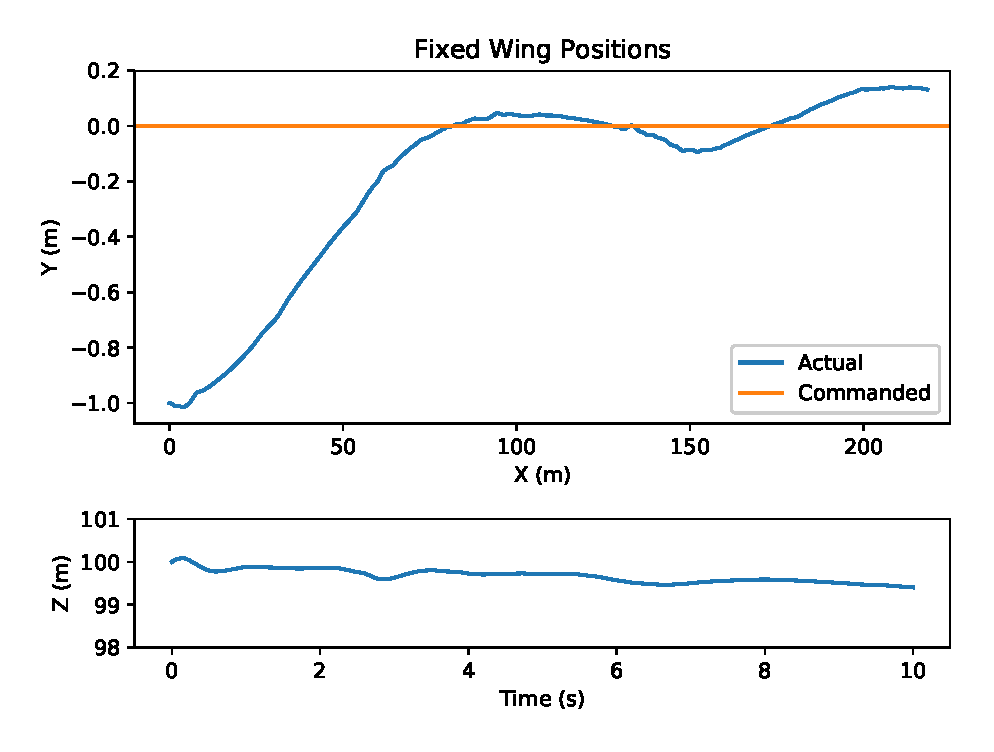
\includegraphics[width=0.45\textwidth]{figures/fixedwing_offset.eps}
		\label{fig:fw_offset_positions}
	}
	\qquad
	\subfloat[]{
		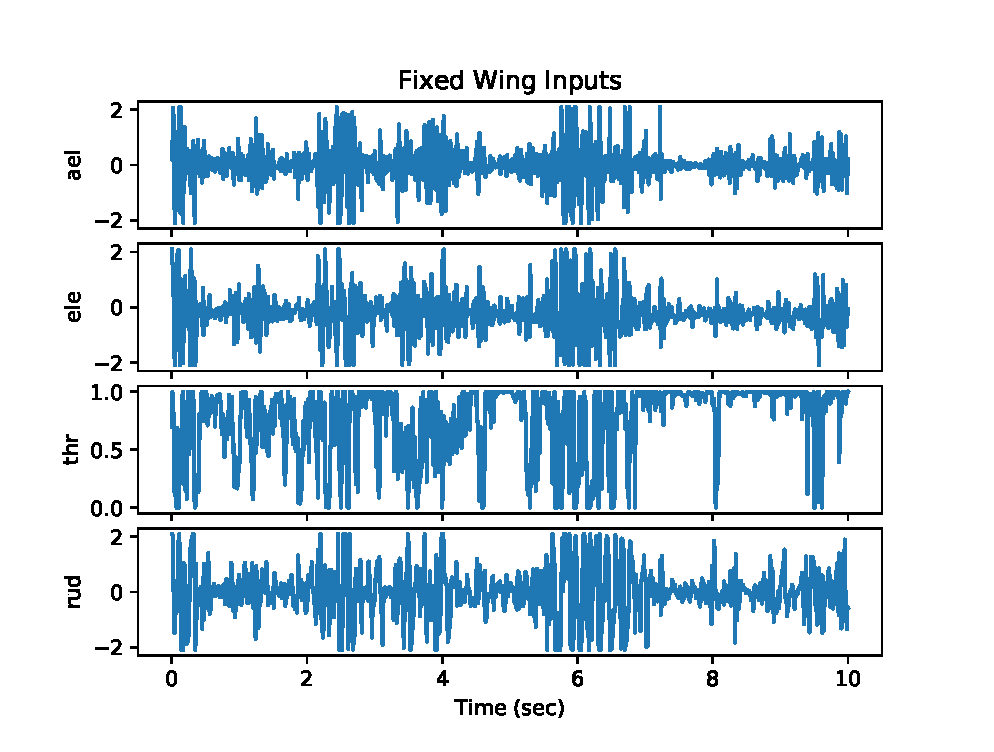
\includegraphics[width=0.45\textwidth]{figures/fixedwing_offset_inputs.eps}
		\label{fig:fw_offset_inputs}
	}
	\caption{Case 2 is the optimization of the aircraft in level flight but with an initial offset starting point. The aircraft started at the point (0,-1,100) and was commanded to maintain the course on the commanded straight line. It took 120.64 seconds to run 10 seconds of simulation.}
	\label{fig:fw_offset}
\end{figure*}


\begin{figure*}[htbp]
	\centering
	\subfloat[]{
		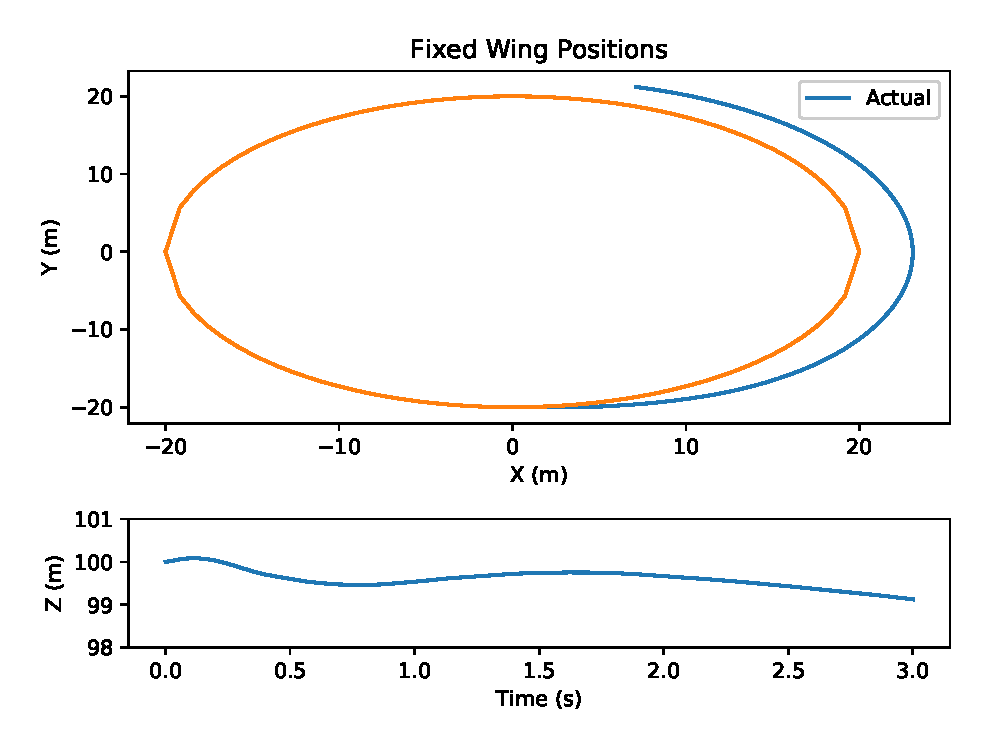
\includegraphics[width=0.45\textwidth]{figures/fixedwing_circle.eps}
		\label{fig:fw_circle_positions}
	}
	\qquad
	\subfloat[]{
		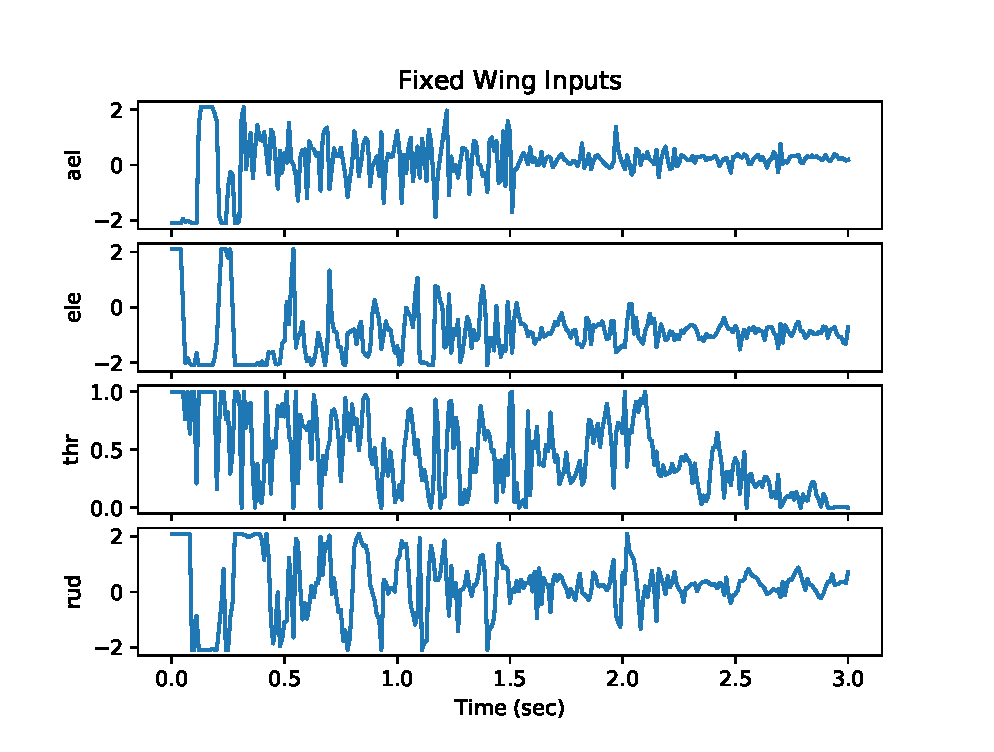
\includegraphics[width=0.45\textwidth]{figures/fixedwing_circle_inputs.eps}
		\label{fig:fw_circle_input}
	}
	\caption{Case 2 is a base case to see if the optimization knows how to keep the aircraft in  flight. It took 37.21 seconds to run 3 seconds of simulation.}
	\label{fig:fw_circle}
\end{figure*}


\begin{appendices}
	
\section{Aircraft Dynamics}
\label{sec:dynamics}

The aircraft's position, velocity, attitude, and angular rate evolve in time according to
\begin{align}
\dot{\mathbf{p}}_{b/I}^{I} & =\left(R_{I}^{b}\right)^{\top}\mathbf{v}_{b/I}^{b}\label{eq:lqr_pdot_true}\\
\dot{\mathbf{v}}_{b/I}^{b} & =\frac{1}{m}\mathbf{f}^{b}-\boldsymbol{\omega}_{b/I}^{b}\times\mathbf{v}_{b/I}^{b}\label{eq:lqr_vdot_true}\\
\dot{\mathbf{q}}_{I}^{b} & =\boldsymbol{\omega}_{b/I}^{b}\label{eq:lqr_qdot_true}\\
\dot{\boldsymbol{\omega}}_{b/I}^{b} & =J^{-1}\left(\boldsymbol{\tau}^{b}-\boldsymbol{\omega}_{b/I}^{b}\times J\boldsymbol{\omega}_{b/I}^{b}\right),\label{eq:lqr_omegadot_true}
\end{align}
where $m$ is the aircraft's mass, $J$ is the aircraft's inertia matrix, and $\mathbf{f}^b$ and $\boldsymbol{\tau}^b$ are the force and torque applied to the aircraft body~\cite{beard2012small}.

We assume that the aircraft is equipped with the four control inputs: aileron, elevator, throttle, and rudder.
The aircraft receives a throttle signal $s_t\in\left[0,1\right]$ and signals for aileron, elevator, and rudder given by
\begin{align}
s_{a} &= \frac{\delta_{a}}{\delta_{a_{max}}}\in\left[-1,1\right] \\
s_{e} &= \frac{\delta_{e}}{\delta_{e_{max}}}\in\left[-1,1\right] \\
s_{r} &= \frac{\delta_{r}}{\delta_{r_{max}}}\in\left[-1,1\right],
\end{align}
where $\delta_*$ denotes deflection angle in radians and $\delta_{*_{max}}$ is the physically defined, maximum angle of deflection.

Vehicle air velocity, air speed, angle of attack, and side slip angle are defined by
\begin{align}
\mathbf{v}_{a/I}^{b} & =\mathbf{v}_{b/I}^{b}-R_{I}^{b}\mathbf{v}_{w/I}^{I}\\
V_{a} & =\norm{\mathbf{v}_{a/I}^{b}} \\
\alpha & =\tan^{-1}\left(\frac{\mathbf{e}_{3}^{\top}\mathbf{v}_{a/I}^{b}}{\mathbf{e}_{1}^{\top}\mathbf{v}_{a/I}^{b}}\right)\\
\beta & =\sin^{-1}\left(\frac{\mathbf{e}_{2}^{\top}\mathbf{v}_{a/I}^{b}}{V_{a}}\right),
\end{align}
where $\mathbf{v}_{w/I}^I$ is the wind velocity expressed in the inertial frame.

Nondimensionalized coefficients of lift and drag are defined by
\begin{align}
C_{L}\left(\alpha\right) & =\left(1-\sigma\left(\alpha\right)\right)\left[C_{L_{0}}+C_{L_{\alpha}}\alpha\right]+\sigma\left(\alpha\right) \\ & \quad \left[2\mathrm{sign}\left(\alpha\right)\sin^{2}\alpha\cos\alpha\right]\nonumber\\
C_{D}\left(\alpha\right) & =C_{D_{p}}+\frac{S\left(C_{L_{0}}+C_{L_{\alpha}}\alpha\right)^{2}}{\pi eb^{2}},
\end{align}
where
\begin{equation}
\sigma\left(\alpha\right) =\frac{1+e^{-M\left(\alpha-\alpha_{0}\right)}+e^{M\left(\alpha+\alpha_{0}\right)}}{\left(1+e^{-M\left(\alpha-\alpha_{0}\right)}\right)\left(1+e^{M\left(\alpha+\alpha_{0}\right)}\right)}.
\end{equation}
Nondimensionalized coefficients of force in the body $x$ and $z$ axes are therefore given by
\begin{align}
C_{X}\left(\alpha\right) & =-C_{D}\left(\alpha\right)\cos\alpha+C_{L}\left(\alpha\right)\sin\alpha\\
C_{X_{q}}\left(\alpha\right) & =-C_{D_{q}}\cos\alpha+C_{L_{q}}\sin\alpha\\
C_{X_{\delta_{e}}}\left(\alpha\right) & =-C_{D_{\delta_{e}}}\cos\alpha+C_{L_{\delta_{e}}}\sin\alpha\\
C_{Z}\left(\alpha\right) & =-C_{D}\left(\alpha\right)\sin\alpha-C_{L}\left(\alpha\right)\cos\alpha\\
C_{Z_{q}}\left(\alpha\right) & =-C_{D_{q}}\sin\alpha-C_{L_{q}}\cos\alpha\\
C_{Z_{\delta_{e}}}\left(\alpha\right) & =-C_{D_{\delta_{e}}}\sin\alpha-C_{L_{\delta_{e}}}\cos\alpha.
\end{align}

Consequently, the force and torque expressed in the body frame are given by
\begin{align}
\mathbf{f}^{b} & =mR_{I}^{b}\mathbf{g}^{I}+\frac{\rho V_{a}^{2}S}{2}\bigg(C_{F}\left(\alpha,\beta\right)+\left.\frac{1}{2V_{a}}C_{F_{\omega}}\left(\alpha\right)\boldsymbol{\omega}_{b/I}^{b}+C_{F_{u}}\left(\alpha\right)\mathbf{u}\right)+\nonumber\\
&\quad\rho S_{prop}C_{prop}\mathbf{e}_{3}^{\top}\mathbf{u}\left(V_{a}+\mathbf{e}_{3}^{\top}\mathbf{u}\left(k_{motor}-V_{a}\right)\right)\cdot\nonumber\left(k_{motor}-V_{a}\right)\mathbf{e}_{1}\nonumber\\
\boldsymbol{\tau}^{b} & =\frac{\rho V_{a}^{2}S}{2}C_{bc}\bigg(C_{\tau}\left(\alpha,\beta\right)+\frac{1}{2V_{a}}C_{\tau_{\omega}}\boldsymbol{\omega}_{b/I}^{b}+ C_{\tau_{u}}\mathbf{u}\bigg)-k_{T_{p}}\left(k_{\Omega}\mathbf{e}_{3}^{\top}\mathbf{u}\right)^{2}\mathbf{e}_{1},\nonumber
\end{align}
where
\begin{align}
\mathbf{u} & =\begin{bmatrix}s_{a} & s_{e} & s_{t} & s_{r}\end{bmatrix}^{\top}\\
C_{F}\left(\alpha,\beta\right) & =\begin{bmatrix}C_{X}\left(\alpha\right)\\
C_{Y_{0}}+C_{Y_{\beta}}\beta\\
C_{Z}\left(\alpha\right)
\end{bmatrix}\\
C_{F_{\omega}}\left(\alpha\right) & =\begin{bmatrix}0 & C_{X_{q}}\left(\alpha\right)c & 0\\
C_{Y_{p}}b & 0 & C_{Y_{r}}b\\
0 & C_{Z_{q}}\left(\alpha\right)c & 0
\end{bmatrix}\\
C_{F_{u}}\left(\alpha\right) & =\begin{bmatrix}0 & C_{X_{\delta_{e}}}\left(\alpha\right)\delta_{e_{max}} & 0 & 0\\
C_{Y_{\delta_{a}}}\delta_{a_{max}} & 0 & 0 & C_{Y_{\delta_{r}}}\delta_{r_{max}}\\
0 & C_{Z_{\delta_{e}}}\left(\alpha\right)\delta_{e_{max}} & 0 & 0
\end{bmatrix}\\
C_{bc} & =\begin{bmatrix}b & 0 & 0\\
0 & c & 0\\
0 & 0 & b
\end{bmatrix}\\
C_{\tau}\left(\alpha,\beta\right) & =\begin{bmatrix}C_{l_{0}}+C_{l_{\beta}}\beta\\
C_{m_{0}}+C_{m_{\alpha}}\alpha\\
C_{n_{0}}+C_{n_{\beta}}\beta
\end{bmatrix}\\
C_{\tau_{\omega}} & =\begin{bmatrix}C_{l_{p}}b & 0 & C_{l_{r}}b\\
0 & C_{m_{q}}c & 0\\
C_{n_{p}}b & 0 & C_{n_{r}}b
\end{bmatrix}\\
C_{\tau_{u}} & =\begin{bmatrix}C_{l_{\delta_{a}}}\delta_{a_{max}} & 0 & 0 & C_{l_{\delta_{r}}}\delta_{r_{max}}\\
0 & C_{m_{\delta_{e}}}\delta_{e_{max}} & 0 & 0\\
C_{n_{\delta_{a}}}\delta_{a_{max}} & 0 & 0 & C_{n_{\delta_{r}}}\delta_{r_{max}}
\end{bmatrix}.
\end{align}

\end{appendices}


\bibliographystyle{unsrt}
\bibliography{references} % bibliography data in references.bib
\bibliographystyle{IEEEtran}

\end{document}
